There exist two popular datasets in the remote sensing community are the Samson and Salinas dataset. 

% https://aviris.jpl.nasa.gov/
The Salinas is a 512-by-217 hyperspectral image collected by the 224-band AVIRIS sensor over Salinas Valley, California, and is characterized by high spatial resolution (3.7-meter pixels) with spectral wavelengths from 400 to 2500 nanometers. 20 spectral bands were removed from the image corresponding to high-noise channels, resulting in a total of 204 captured spectral bands. The image is comprised of 16 classifications based on various vegetation and vineyard types. [REF] 
\begin{figure}[H]
    \centering
    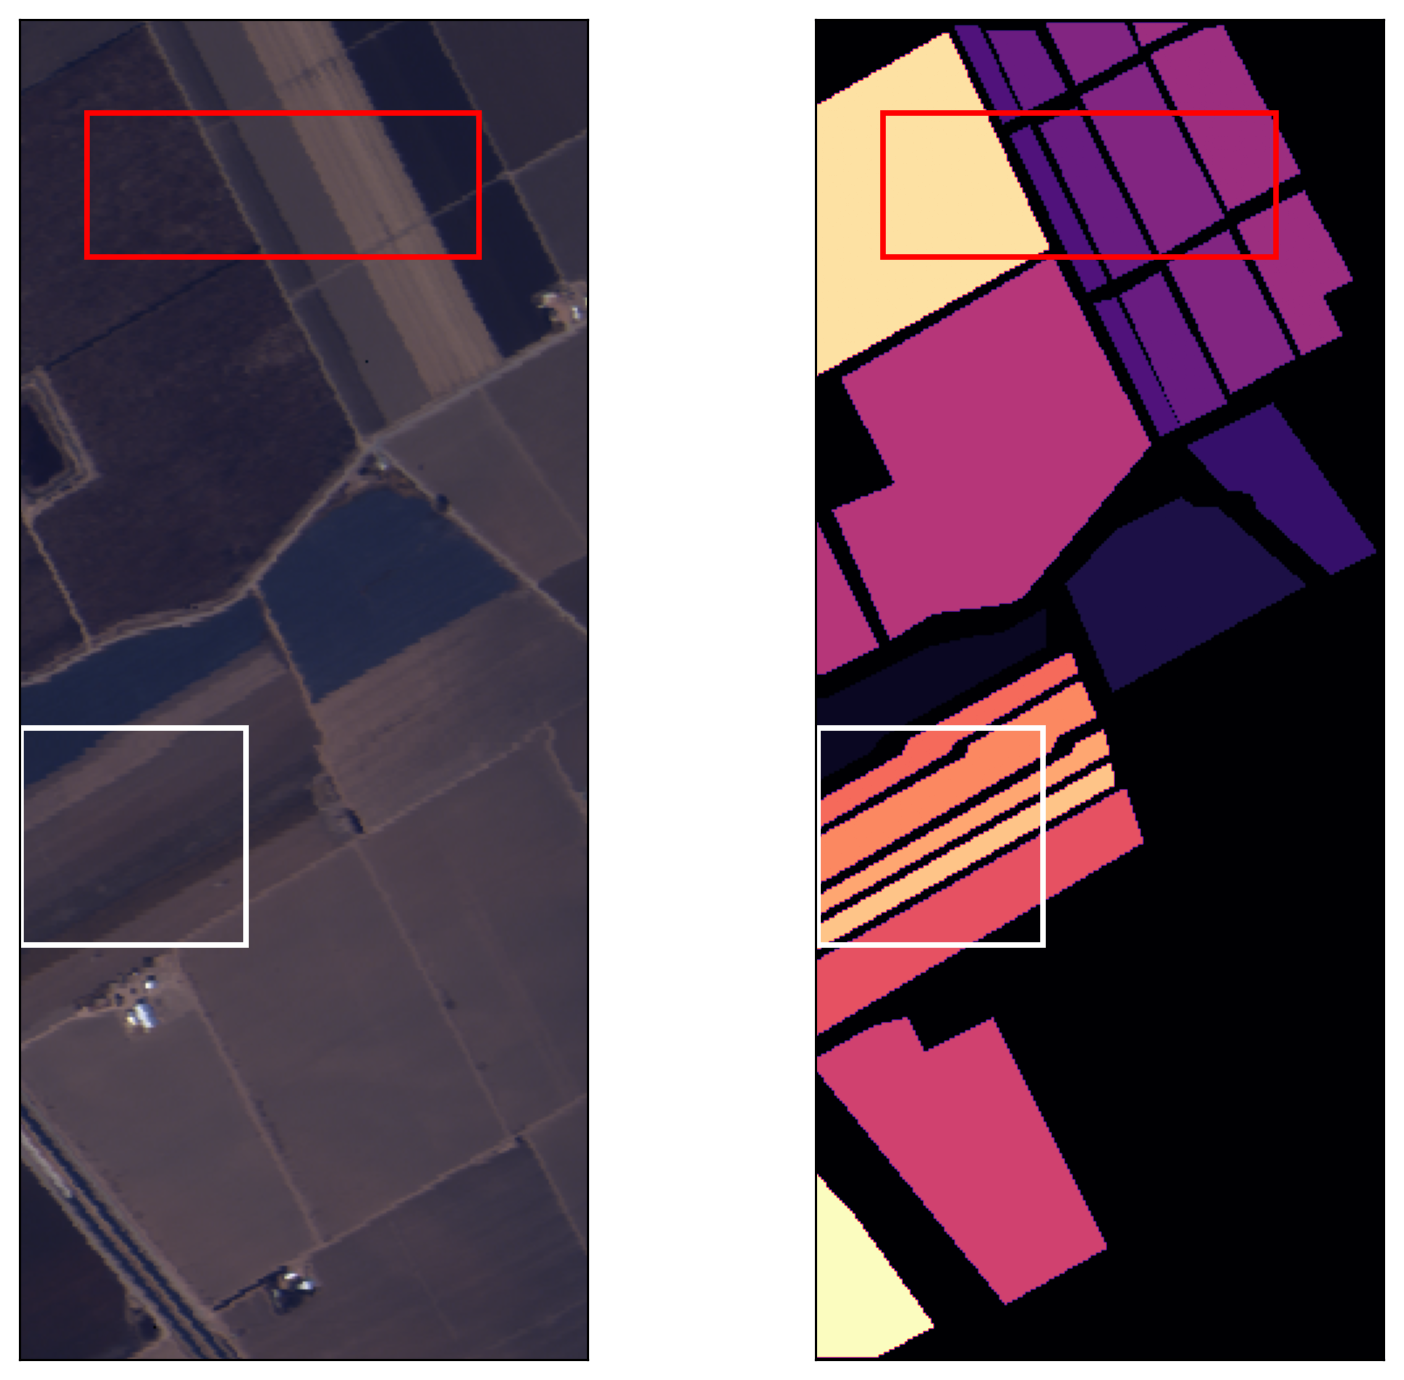
\includegraphics[width=10cm]{salinas_overview.png}  % Adjust width and filename
    \caption{Colorized Salinas \& Ground Truth Labels with Subsets A (White Box) \& B (Red Box)}
    \label{salinas-borders}  % Optional label for referencing
  \end{figure}

The Salinas dataset is commonly used in hyperspectral classification evaluation due to the availibility of ground truth labels within the image. Due to similar spectral characteristics of multiple vegetation types in the image, this dataset is optimal to test the efficacy of the proposed algorithm in segmentation tasks. There are two subsets of the Salinas commonly used for evaluation. Salinas A is a 86-by-83 pixel subset of the Salinas image beginning from pixel index $(270, 0)$ with 6 classifications. Salinas B is a 55-by-150 pixel subset of the Salinas image beginning from pixel index $(35, 25)$ with 5 classifications. Both subsections provide an adequate mix of vegetation types.
\begin{figure}[H]
    \centering
    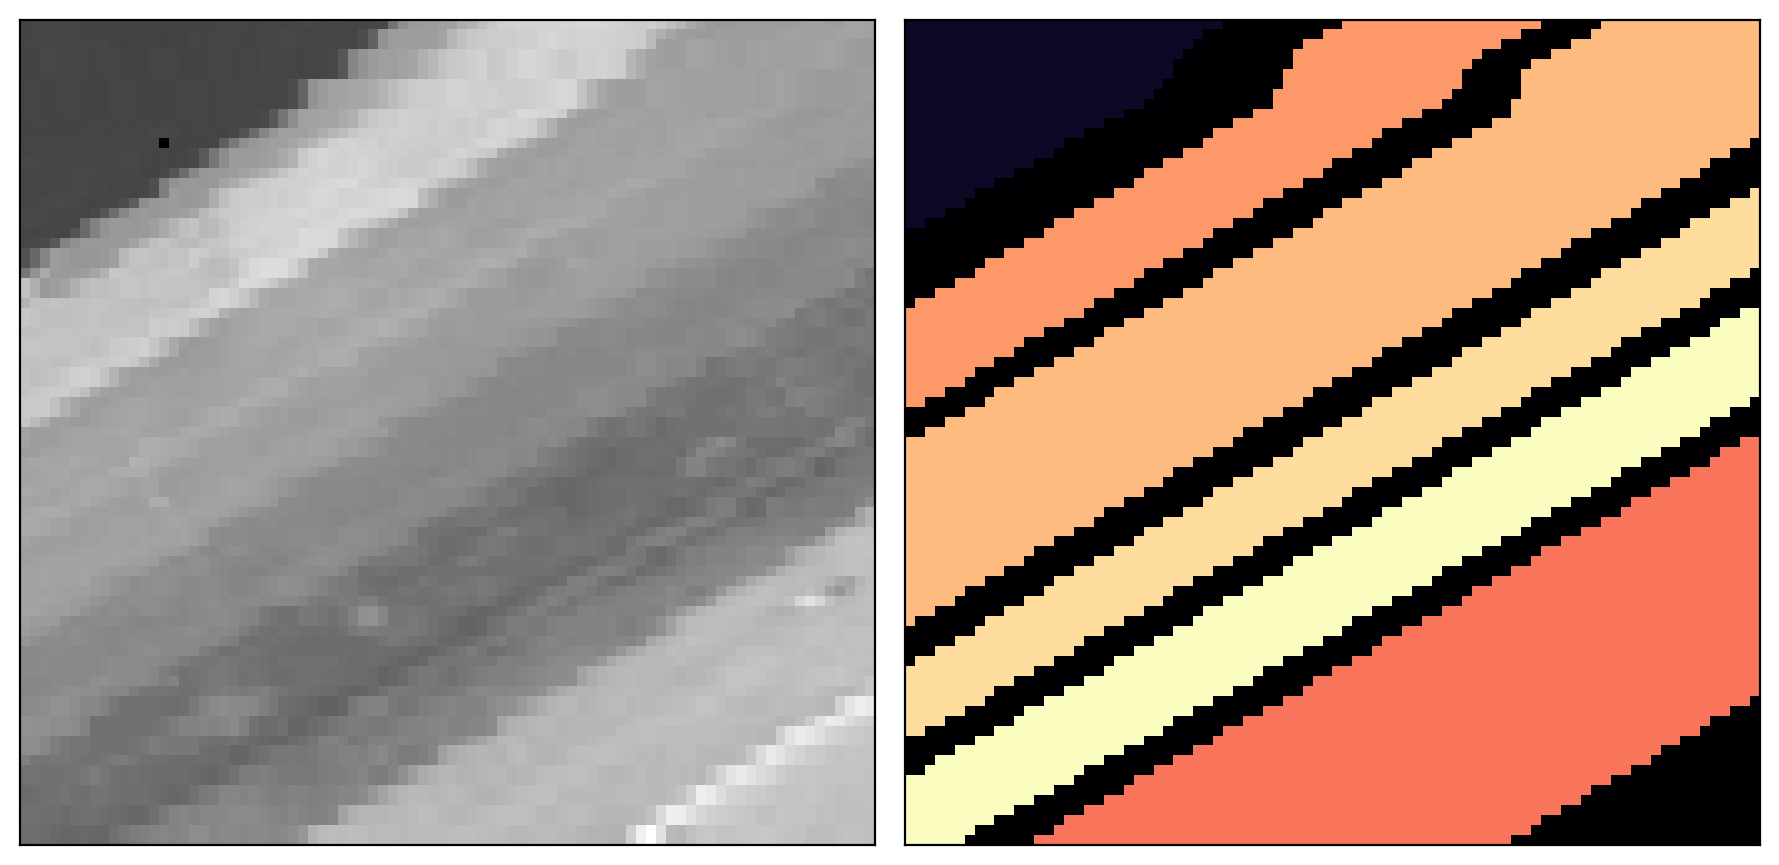
\includegraphics[width=8cm]{salinas-a.png}  % Adjust width and filename
    \caption{Greyscale Salinas-A \& Ground Truth Labels}
    % \label{salinas-a}  % Optional label for referencing
    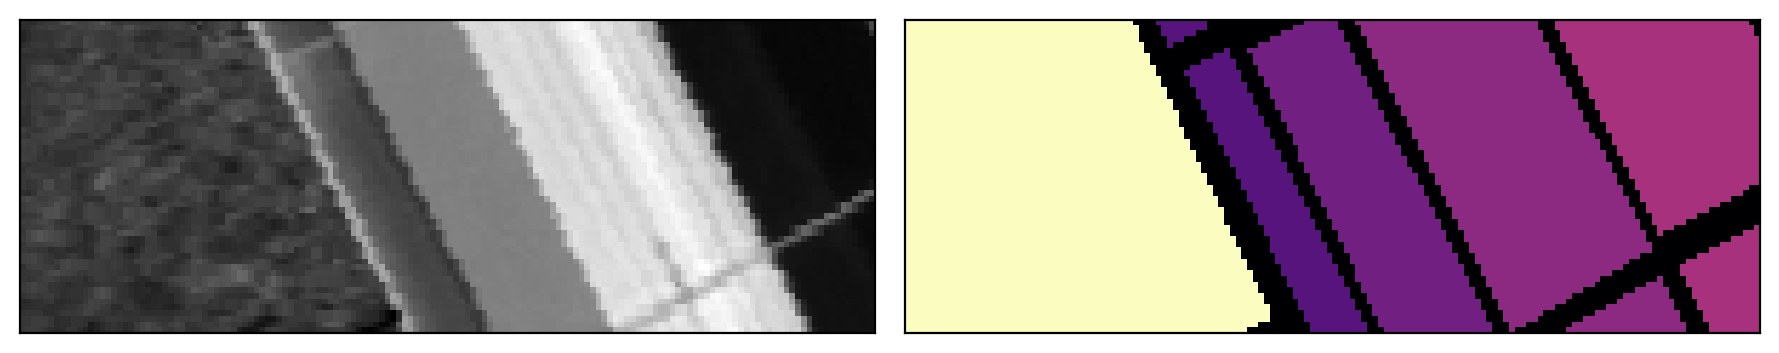
\includegraphics[width=8cm]{salinas-b.png}  % Adjust width and filename
    \caption{Greyscale Salinas-B \& Ground Truth Labels}
    \label{salinas-ab}  % Optional label for referencing
  \end{figure}

In similar fashion, Samson is a 952-by-952 hyperspectral image captured by 156-band SAMSON sensor over Elkhorn, California. The image covers a spectral range of 400nm to 900nm with a bandwidth of 3.2nm. This image does not include any ground truth classification, however subsets of the image are created comprised of soil, trees, and water. [REF]
\begin{figure}[H]
  \centering
  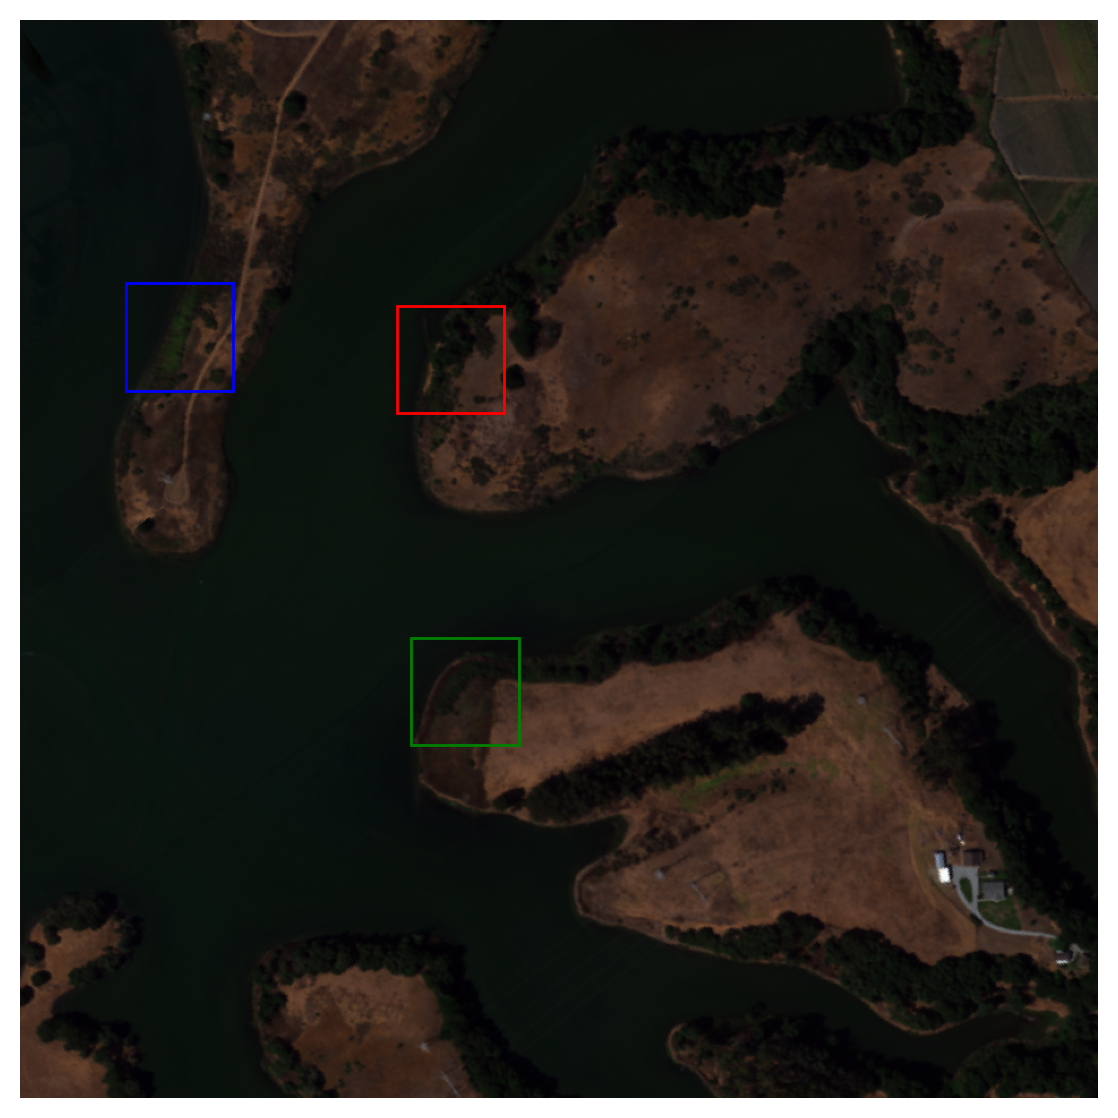
\includegraphics[width=10cm]{samson_full.png}  % Adjust width and filename
  \caption{Colorized Samson \& with Subsets A (Red), B (Blue), C (Green)}
  \label{samson}  % Optional label for referencing
\end{figure}

The Samson-A, Samson-B, Samson-C subsets are all 95-by-95 hyperspectral images of regions originating from pixel indices (332, 252), (93, 232) and (345, 545) respectiely. The subsets are comprised of the shore lines of where there are many mixed pixel measurements occur due the mixing of materials and complex forms created by the distribution of materials.
\begin{figure}[H]
  \centering
  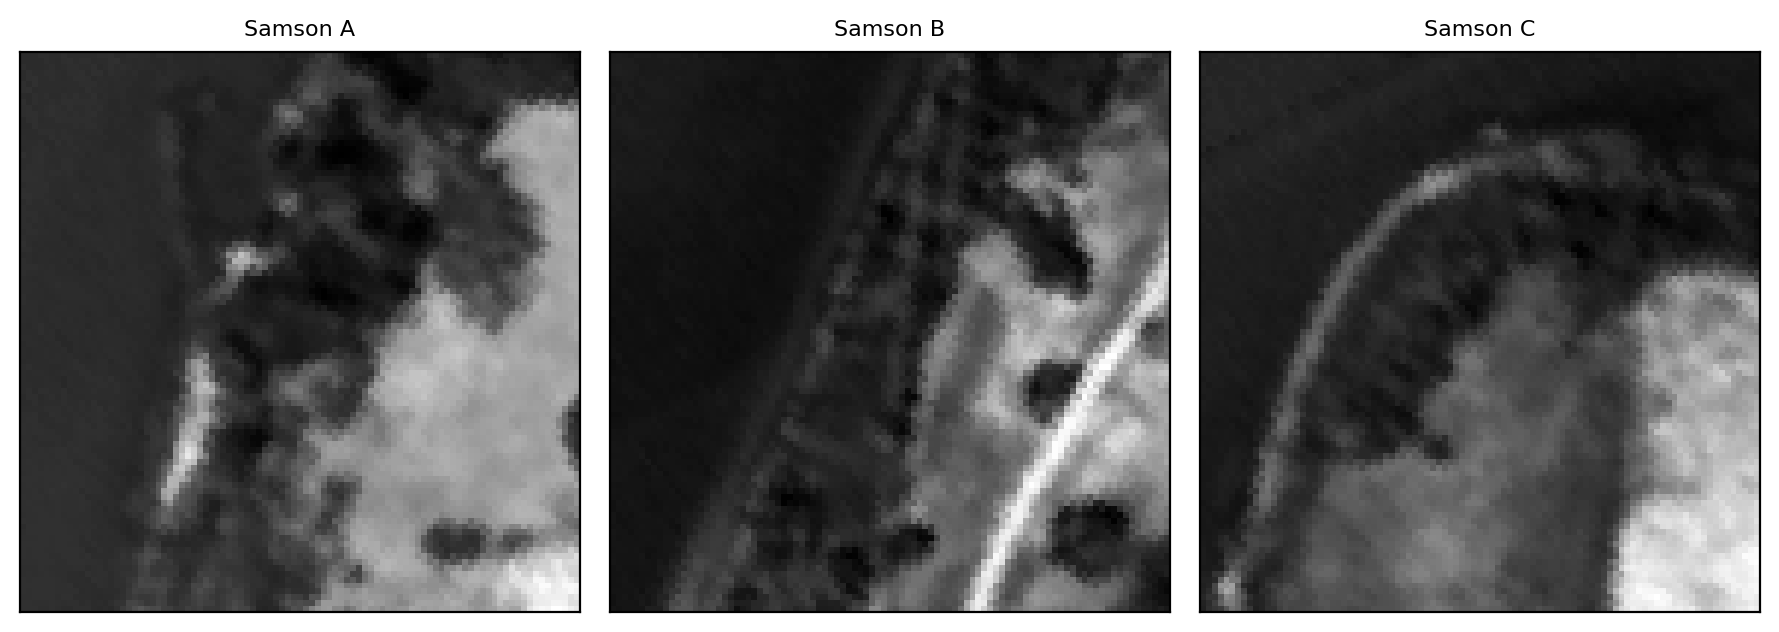
\includegraphics[width=15cm]{samsonabc.png}  % Adjust width and filename
  \caption{Greyscale Samson Subsets}
  \label{samsonabc}  % Optional label for referencing
\end{figure}


